\section{Design Patterns}
  \subsection{Architetturali}
    \subsubsection{Architettura a microservizi}
      \begin{itemize}
       \item \textbf{Scopo:} l'architettura a microservizi è un approccio allo sviluppo di una singola applicazione come insieme di piccoli servizi, ciascuno dei quali viene eseguito da un proprio processo e comunica con un meccanismo snello, spesso una HTTP API;
       \item \textbf{Vantaggi:}
	      \begin{itemize} 
	       \item ogni microservizio è relativamente piccolo, quindi più semplice da implementare e da capire per gli sviluppatori;
	       \item ogni microservizio è indipendente dagli altri; è quindi possibile distribuire nuove versioni più frequentemente e isolare i possibili errori.
	      \end{itemize}

       \item \textbf{Svantaggi:}
	\begin{itemize}
	 \item l'architettura risulta maggiormente complessa perchè risulta essere un sistema distribuito;
	 \item la gestione di più microservizi potrebbe risultare in un carico di lavoro maggiore rispetto ad una sua versione monolitica.
	\end{itemize}
       \item \textbf{Utilizzo:}
      \end{itemize}
      \begin{figure}[h]
      	\centering
      	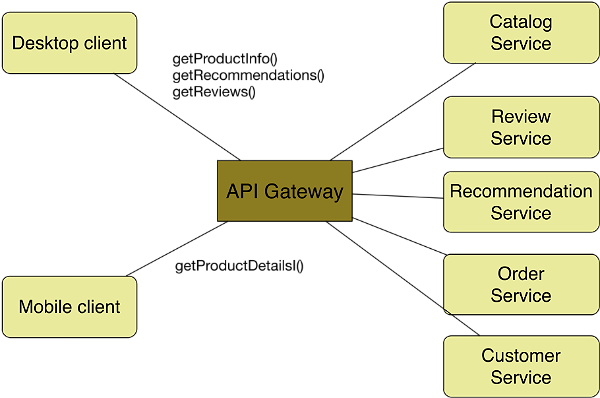
\includegraphics[width=\textwidth,height=\textheight,keepaspectratio,scale=0.1]{images/apigateway1.png}
      	\caption{Architettura a microservizi}\label{fig:micr1}
      \end{figure}
    \subsubsection{Architettura event-driven}
      \begin{itemize}
       \item \textbf{Scopo:} anche se non è un vero e proprio pattern, l'architettura event-driven è un particolare tipo di architettura asincrona per sistemi distribuiti basata sugli eventi.
	\item \textbf{Vantaggi:}
	  \begin{itemize}
	   \item per definizione, questo tipo di architettura è particolarmente adatto ad ambienti di tipo asincrono basati sugli eventi, come ad esempio l'interazione con degli utenti in tempo reale.
	  \end{itemize}
	\item \textbf{Svantaggi:}
	  \begin{itemize}
	   \item i sistemi che utilizzano tale architettura sono spesso distribuiti: ciò comporta un maggiore livello di complessità.
	  \end{itemize}
	\item \textbf{Utilizzo:}
	\end{itemize}
     
     \subsubsection{Client-side discovery}
      \begin{itemize}
       \item \textbf{Scopo:} all'interno di un'architettura a microservizi, i singoli microservizi si trovano spesso in posizioni non fissate in quanto decise dinamicamente. Un metodo per la loro localizzazione consiste nel pattern Client-side discovery, che consiste nella richiesta della posizione di uno specifico microservizio da parte del client ad un registro, che conosce le posizioni di tutte le istanze dei microservizi. 
	\item \textbf{Vantaggi:}
	  \begin{itemize}
	   \item permette di allocare dinamicamente diverse istanze di diversi servizi.
	  \end{itemize}
	\item \textbf{Svantaggi:}
	  \begin{itemize}
	   \item crea dipendenze tra il registro e il client.
	  \end{itemize}
	\item \textbf{Utilizzo:}
	\end{itemize}

    
   \subsubsection{Data Access Object}
      \begin{itemize}
       \item \textbf{Scopo:} il pattern Data Access Object (DAO) consiste nell'utilizzo di un oggetto che fornisce un'interfaccia astratta per la gestione di ua sorgente di dati, o più in generale per la gestione della persistenza.
	\item \textbf{Vantaggi:}
	  \begin{itemize}
	   \item separazione tra logica di business e dati;
	   \item modifiche sul dati non comportano modifiche sul client cche utilizza DAO.
	  \end{itemize}
	\item \textbf{Svantaggi:}
	  \begin{itemize}
	   \item un'interfaccia di questo tipo potrebbe nascondere i costi di accesso ad un database;
	   \item potrebbe essere necessarie molte più operazioni rispetto all'esecuzione diretta di una query su un database.
	  \end{itemize}
	\item \textbf{Utilizzo:}
	\end{itemize}
	\begin{figure}[h]
		\centering
		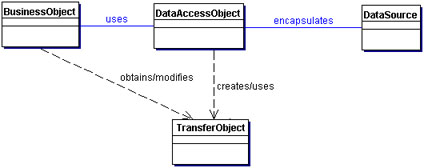
\includegraphics[width=\textwidth,height=\textheight,keepaspectratio,scale=0.1]{images/DAOpattern.jpg}
		\caption{pattern Data Access Object (DAO)}\label{fig:dao1}
	\end{figure}
	\newpage	
    \subsubsection{Dependency Injection}
     \begin{itemize}
       \item \textbf{Scopo:} consiste nella separazione del comportamento di una componente dalla risoluzione delle sue dipendenze.
	\item \textbf{Vantaggi:}
	  \begin{itemize}
	   \item la separazione del comportamento dalle dipendenze rende una componente molto più flessibile;
	   \item rende le singole componenti maggiormente indipendenti permettendo una più facile progettazione dei test di unità.
	  \end{itemize}
	\item \textbf{Svantaggi:}
	  \begin{itemize}
	   \item eventuali errori legati alla risoluzione delle dipendenze o alla loro implementazione vengono rilevati solamente a runtime;
	   \item rende più difficile il tracciamento del codice in quanto ne separa la costruzione dal comportamento.
	  \end{itemize}
	\item \textbf{Utilizzo:}
	\end{itemize}
  
  \subsection{Strutturali}
  
    \subsubsection{Facade}
      \begin{itemize}
       \item \textbf{Scopo:}  indica un oggetto che permette, attraverso un'interfaccia più semplice, l'accesso a sottosistemi che espongono interfacce complesse e molto diverse tra loro, nonché a blocchi di codice complessi. 
	\item \textbf{Vantaggi:}
	  \begin{itemize}
	   \item permette di nascondere la complessità di un'operazione: rispetto alla chiamata diretta di un sottoinsieme di classi è possibile chiamare solamente la classe definita come facade semplificando l'operazione;
	   \item permette di diminuire le dipendenze tra sottosistemi;
	  \end{itemize}
	\item \textbf{Svantaggi:}
	  \begin{itemize}
	   \item i sottosistemi risultano essere collegati al facade: modifiche alla struttura dei sottosistemi comportano una serie di modifiche al facade stesso;
	  \end{itemize}
	\item \textbf{Utilizzo:}
	\end{itemize}
	
    \subsubsection{Adapter}
      \begin{itemize}
       \item \textbf{Scopo:} questo pattern permette la comunicazione tra due interfacce completamente differenti tramite l'utilizzo di un Adapter.
	\item \textbf{Vantaggi:}
	  \begin{itemize}
	   \item permette la conversione di una classe esistente in un'altra completamente differente senza modificarne il codice;
	   \item maggiore flessibilità nella progettazione.
	  \end{itemize}
	\item \textbf{Svantaggi:}
	  \begin{itemize}
	   \item aumenta la dimensione del codice;
	   \item a volte per interconnettere due interfacce sono necessari più Adapter.
	  \end{itemize}
	\item \textbf{Utilizzo:}
	\end{itemize}
	
  \subsection{Creazionali}
  
    \subsubsection{Singleton}
      \begin{itemize}
       \item \textbf{Scopo:} questo pattern ha lo scopo di garantire che di una determinata classe venga creata una e una sola istanza, e di fornire un punto di accesso globale ad essa.
	\item \textbf{Vantaggi:}
	  \begin{itemize}
	   \item questo pattern risulta molto utile ogni qual volta è necessaria una sola istanza di una classe.
	  \end{itemize}
	\item \textbf{Svantaggi:}
	  \begin{itemize}
	   \item la classe Singleton risulta essere globale, e di conseguenza rende più difficile la definizione di test di unità;
	   \item aumenta il livello di accoppiamento del codice.
	  \end{itemize}
	\item \textbf{Utilizzo:}
	\end{itemize}
	
	 \subsubsection{Module}
      \begin{itemize}
       \item \textbf{Scopo:} questo pattern ha lo scopo di introdurre il concetto di modularità nel linguaggi di programmazione che non lo possiedono.
	\item \textbf{Vantaggi:}
	  \begin{itemize}
	   \item come da definizione, questo pattern permette l'implementazione della modularità in ambienti privi di supporto ad essa.
	  \end{itemize}
	\item \textbf{Svantaggi:}
	  \begin{itemize}
	   \item la sua implementazione richiede un maggiore carico di lavoro.
	  \end{itemize}
	\item \textbf{Utilizzo:}
	\end{itemize}
  \subsection{Comportamentali}
  
    \subsubsection{Observer}
      \begin{itemize}
       \item \textbf{Scopo:} questo pattern permette la definizione di una o più classi Observer le quali "osservano" una classe Soggetto e ne gestiscono gli eventi.
	\item \textbf{Vantaggi:}
	  \begin{itemize}
	   \item permette la gestione di eventi tramite l'invio di dati ad altre classi in modo efficiente;
	   \item la definizione di classi Observer non causa modifiche alla classe Soggetto. 
	  \end{itemize}
	\item \textbf{Svantaggi:}
	  \begin{itemize}
	   \item una cattiva implementazione comporta un aumento della complessità del codice;
	   \item l'interfaccia Observer deve essere implementata, e ciò comporta ereditarietà.
	  \end{itemize}
	\item \textbf{Utilizzo:}
	\end{itemize}
	
	\section{Tecnologie utilizzate}
	\subsection{Promise e Observable}


JavaScript è un linguaggio single-thread, quindi basato su un singolo thread in esecuzione. Questo significherebbe dover aspettare sempre il termine di un'operazione prima di passare alla

successiva, quindi nel caso di operazioni di lunga durata, il flusso dell'elaborazione principale di un’applicazione JavaScript potrebbe "congelarsi". \\


Per aggirare questo problema, una delle soluzioni più diffuse è quella di passare una callback alla funzione in questione e, anzichè aspettare il compimento dell'operazione, restituisce

il controllo al chiamante. Quando l'operazione sarà terminata, la funzione di callback verrà invocata. \\


L'uso di callback, spesso annidate, rendono il codice di difficile comprensione e di difficile manutenzione. Due possibili soluzioni sono l'uso delle Promise di bluebird e gli Observable

di RxJS.


\subsubsection{Promise e bluebird}

Una Promise è un oggetto che rappresenta il risultato pendente di un’operazione asincrona. Ciò permette ai metodi asincroni di restituire valori alla stessa maniera dei metodi sincroni:
invece del valore finale, il metodo asincrono restituisce una promessa di ottenere un valore in un momento futuro. \\
I principali metodi di una Promise sono:

\begin{itemize}

\item then: ritorna una Promise, in questo modo è possibile concatenere successive chiamate a questo meotodo. È composto da due parametri opzionali che corrispondono a 

due funzioni: onFulfill viene richiamata se la Promise ha avuto successo, onReject se è stata rigettata.  

\item catch: ritorna una Promise e si occupa di gestire eventuali errori generati nella catena dei then.

\end{itemize}


Si è deciso di utilizzare bluebird in quanto offre le suguenti caratteristiche:

\begin{itemize}

\item cross-platform: ideale per progetti che prevedono esperienze multipiattaforma;

\item compatibile con le specifiche Promise/A+: bluebird può essere usato come rimpiazzo per Promise nativa offrendo un immediato miglioramento delle prestazioni;

\item debug facile: gli stake trace sono in cui vengono riportati, quando possibile, gli errori non gestiti sono configurabili.

\end{itemize}


\subsubsection{Observable e RxJS v5}

Un Observable è una rappresentazione di un qualsiasi insieme di valori durante un qualsiasi periodo di tempo. Viene utilizzata per le implementazioni del pattern Observer.

RxJS v5 è ancora in beta ma sostituirà in breve la v4. Si è deciso di utilizzarla perchè è una libreria solida nella gestione degli Observable e sarà ulteriormente aggiornta

da Microsoft e altri sviluppatori di software open source.


\subsection{AWS SDK per JavaScript in Node.js}

Siccome il gruppo ha deciso di appoggiarsi all'infrastruttura Amazon Web Services (AWS) per lo sviluppo del sistema è necessario utilizzare SDK per JavaScript in Node.js per

interfacciarsi ai singoli servizi offerti da AWS. In particolare si farà utiizzo di DynamoDb.


\subsubsection{Node.js}
La parte Back-End è stata sviluppata tramite la piattaforma event-driven Node.Js, basata sul motore JavaScript V8. Esso permette di realizzare applicazioni Web utilizzando JavaScript, tipicamente client-side, per la scrittura server-side. La caratteristica principale di Node.js risiede nella possibilità che offre di accedere alle risorse del sistema operativo in modalità event-driven non sfruttando il classico modello basato su processi o thread concorrenti, utilizzato dai classici web server.

\subsubsection{AWS Lambda}
AWS Lambda è un servizio di elaborazione serverless che esegue codice in risposta a determinati eventi e gestisce automaticamente le risorse di elaborazione in uso. Può essere usato per estendere altri servizi AWS con logica personalizzata oppure creare servizi di back-end.  

\subsubsection{Serverless Framework}
Serverless Framework è un web framework gratuito e open-source scritto tramite Node.js. Serverless è un framework per creare applicazioni esclusivamente su AWS Lambda. Un applicazione Serverless può essere composta da poche lambda functions per portare a termine semplici tasks o da molte lambda functions per creare ad esempio un intero back-end.

\subsubsection{DynamoDB}
Amazon DynamoDB è un servizio database NoSQL, il quale permette di immagazzinare documenti e grafici tra i suoi dati. E' veloce e flessibile, ideato per tutte le applicazioni che richiedono una latenza costante non superiore a una decina di millisecondi, e grazie alle sue caratteristiche si presta perfettamente come supporto per applicazioni Web.

\subsubsection{API.AI}
API.AI è una piattaforma di conversazione che permette interazioni sofisticate con il linguaggio naturale.
Le applicazioni sviluppate su questa piattaforma sono costuite da Agent, i quali si occupano di trasformare il linguaggio naturale in dati processabili. Tali Agent sono a loro volta costituiti da Intent, che hanno il compito di associare la richiesta dell'utente ad una determinata azione del software, ed Entity, che sono strumenti per estrarre dal linguaggio naturale i parametri attesi.

\subsubsection{JWT}
JWTè uno standard basato su JSON per creare token di accesso che possono sostenere richieste. I token sono firmati dalla chiave del server, quindi il client può verificare se un token è legittimo. I token sono pensati per essere compatti, senza contenere caratteri invalidi per gli URL e usabili principalmente nei contesti Single sign-on (SSO).Le richieste JWT possono essere usate solitamente per passare l'identità di un utente autenticato tra un identity provider e un service provider. I token inoltre possono essere autenticati e criptati.

\subsubsection{Web Speech API}
Web Speech API fornisce fornisce due aree distinte di funzionalità, il riconoscimento vocale e la sintesi vocale (conosciuta anche come text to speech o tts).
Il riconoscimento vocale è acceduto attraverso l'interfaccia SpeechRecognition, la quale fornisce la possibilità di riconoscere il contesto vocale da un input vocale e risponde appropriatamente. 
La sintesi vocale è acceduta tramite l'interfaccia SpeechSynthesis, una componente text-to-speech che permette ai programmi di leggere testo.

\subsubsection{Speaker recognition}
Speaker Recognition API è un servizio Microsoft che identifica utenti individual, e li autentica per mezzo della voce. Al suo interno utilizza JSON per lo scambio dei dati e API Keys per l'autenticazione.

\subsubsection{STT IBM Watson}
Lo Speech to Text Watson converte voce in testo scritto. Per trascrivere la voce umana accuratamente il servizio utilizza il machine learning per combinare informazioni riguardo la grammatica e la struttura del linguaggio con la composizione del segnale audio. Il servizio fornisce trascrizioni sempre migliori in base a quanto dialogo viene ascoltato.

\subsubsection{Request promise}
E' un modello che implementa l'esistenza delle Promises come risposta a una serie di richieste che non possono essere soddisfatte immediatamente . Una promessa è un risultato che verrà reso disponibile non appena possibile se è possibile mantenere la promessa (fulfilled) oppure è un errore se non la si può mantenere (rejected).
\subsubsection{AWS Lambda}
AWS Lambda è un servizio di cloud-computing fornito da Amazon, il quale permette l'implementazione di una architettura serverless. \\
Esso permette l'esecuzione di codice senza preoccuparsi della gestione di server o di tutte le risorse necessarie all'esecuzione del codice, in termini di tempo, spazio e computabilità. \\
AWS Lambda permette di eseguire codice su una piattaforma ad alta affidabilità, a patto che il codice sia scritto in un linguaggio supportato. Nel nostro caso, faremo utilizzo di Node.js 4.3.2, supportato da AWS Lambda. \\
Inoltre, questo servizio può essere utilizzato per eseguire del codice in risposta ad eventi. \\
La signature delle Lambda Function è la seguente:
\begin{verbatim}
function(event, context,) {
    ...
}
\end{verbatim}
dove:
\begin{itemize}
	\item \file{event} è l'oggetto che contiene i dati della richiesta ricevuta dall'API Gateway. In particolare, contiene i seguenti campi:
	\begin{itemize}
		\item \file{body}: campo di tipo \file{String} contenente il corpo della richiesta;
		\item \file{pathParameters}: oggetto contenente i parametri passati all'API Gateway attraverso il path dell'URL;
		\item \file{urlQueryParameters}: oggetto contenente i parametri passati all'API Gateway attraverso query nell'URL.
	\end{itemize}
	\item \file{context} è l'oggetto contenente i dati relativi alla richiesta e, in caso di Lambda Proxy Integration, contiene anche i seguenti metodi:
	\begin{itemize}
		\item \file{succeed}: metodo da utilizzare per mandare una risposta all'API Gateway in caso di successo. La risposta dev'essere un oggetto contenente i seguenti campi:
		\begin{itemize}
			\item \file{headers}: array associativo nel quale la chiave indica il nome di un header HTTP da mandare nella risposta, il quale valore associato è una stringa contenente il valore di tale header;
			\item \file{statusCode}: attributo intero contenente il codice HTTP che dovrà avere la risposta;
			\item \file{body}: stringa contenente il corpo della risposta da mandare.  
		\end{itemize}
	\end{itemize} – AWS Lambda uses this parameter to provide your handler the runtime information of the Lambda function that is executing. For more information, see The Context Object (Node.js).
\end{itemize}

